\documentclass[twocolumn,11pt,a4paper]{article}

\usepackage[utf8]{inputenc}
\usepackage[T1]{fontenc}
\usepackage{lmodern}
\usepackage{amsmath,amssymb,amsfonts}
\usepackage{graphicx}
\usepackage{booktabs}
\usepackage{siunitx}
\usepackage{hyperref}
\usepackage{tikz}
\usepackage{pgfplots}
\pgfplotsset{compat=1.17}
\usepackage{caption}
\usepackage{subcaption}
\usepackage{geometry}
\geometry{a4paper, top=2cm, bottom=2cm, left=2cm, right=2cm}

\title{\textbf{Human Consciousness Can Construct the Universe:\\
A Chiral Coarse-Quantum Framework and Testable Predictions}}
\author{Xiaohui Li\\
Independent Researcher, Baoji, China\\
\texttt{danceluck@163.com}\\
ORCID: 0009-0003-8233-7191\\
Data \& code: \url{https://github.com/xiaohui-li-lab/}}
\date{}

\begin{document}

\twocolumn[
\begin{@twocolumnfalse}
\maketitle

\begin{abstract}
The ability of human language to describe both the microscopic quantum world and the macroscopic cosmos has usually been treated as a contingent fact of culture or cognition. Here we propose that this descriptive power reflects a deeper organizational continuity: language, quantum matter, and the large-scale universe may all share a common chiral template. We introduce the Chiral Coarse-Quantum Framework (CCQF), which posits that consciousness is not an emergent property of matter, nor a phenomenon confined within the universe, but a trans-universal, pre-geometric field of information integration that is extremely weak, non-local, and not necessarily chiral in itself. Its relationship to physics is proposed to occur through the initial singularity---a mathematical point that serves as the simplest interface between an unextended consciousness and a finite physical cosmos. After the originating event, the universe expands from a chirally symmetric state; a minute perturbation tips the balance and triggers self-amplifying homochiral attraction, producing the left-handed dominance later observed in weak interactions and, possibly, in cosmic structure. Human language, continuously coupled to consciousness and embedded in a chiral universe, is hypothesized to inherit a left-handed helical bias in its syntactic architecture. We derive four testable predictions---concerning large-scale cosmic helicity, right-handed neutrino abundance, syntactic chirality across languages, and parity-violation phase transitions in cold chiral condensates---and provide an open-source computational toolkit with rigorous benchmarks against exact results. If confirmed, it would offer a unified origin story for cosmic homochirality, quantum parity violation, and the representational capacity of human language.
\end{abstract}

\textbf{Keywords:} consciousness; chirality; cosmic homochirality; language origins; quantum cosmology; parity violation.

\vspace{1em}
\end{@twocolumnfalse}
]

\section{Introduction}

Human beings routinely use finite symbolic systems---languages---to speak about electrons, DNA, galaxies, and the Big Bang. That a biological product of one planet should be able to represent structures spanning twenty orders of magnitude in scale is remarkable, yet it is usually explained by invoking convention, abstraction, and neural computation. These explanations are sufficient for many purposes, but they leave a structural question unanswered: why should the formal organization of language be compatible with the formal organization of the physical world at all?

A clue comes from one of the most striking features of nature: chirality. The weak interaction violates parity~\cite{lee1956, wu1957}; the Standard Model is built on a left-handed electroweak doublet~\cite{glashow1970, weinberg1967}; and life on Earth uses left-handed amino acids and right-handed sugars~\cite{vester1959, soai1995}. Chirality is not a decorative feature---it is woven into the fabric of physics and biology. We therefore ask whether chirality might also be woven into the fabric of human language, and whether this shared chirality could explain why language can represent both quantum and cosmic phenomena.

We propose the Chiral Coarse-Quantum Framework (CCQF). Its central claim is that consciousness is not produced by the brain and is not located inside the universe. It is a trans-universal, pre-geometric field of information integration that is extremely weak, non-local, and not necessarily chiral in itself. The field's contact with physics is the initial singularity: a mathematical point that is the natural interface between an unextended consciousness and a finite cosmos. The universe begins in a chirally symmetric state; a tiny perturbation breaks the symmetry, and self-amplifying homochiral attraction drives the cosmos into a left-handed vacuum. Life and language arise within this chiral universe and retain its organizational signature. Language can describe the world because, at the level of chiral geometry, language and world are cut from the same cloth.

This paper is organized as follows. Section~\ref{sec:framework} presents the conceptual framework. Section~\ref{sec:model} formalizes a chiral spin-network model and benchmarks it against the exact two-dimensional Ising critical temperature. Section~\ref{sec:predictions} derives four testable predictions, with numerical validation and proposed datasets. Section~\ref{sec:discussion} discusses implications and limitations.

\section{Conceptual framework}
\label{sec:framework}

\subsection{Consciousness and the singularity}

In CCQF, consciousness is defined operationally as a pre-geometric field capable of integrating information without being itself a physical object in space or time. It is taken to be trans-universal: it is not inside the universe, because anything that can represent or ``contain'' the universe in thought cannot be merely one more object within it~\cite{wheeler1983, tononi2016}. It is also extremely weak and non-local; its direct effect on ordinary matter is negligible under most conditions.

The most natural point of contact between such a field and physical reality is a mathematical point---the initial singularity. A point has no extension, no chirality, and no internal structure; it is the simplest boundary at which an unextended consciousness can seed a finite cosmos. We therefore hypothesize that the singularity is not a random fluctuation but the place where the trans-universal field actualizes the physical universe.

\subsection{Chiral genesis of the universe}

The nascent universe is assumed to begin in a chirally symmetric state, with left-handed and right-handed quantum modes in equal proportion. Because opposite chiralities are mutually repulsive, this symmetric state is highly unstable and manifests as the Big Bang. A minute perturbation---of magnitude $\eta \ll 1$---favors one handedness. The same-chirality modes then attract one another, and the small initial excess is amplified into macroscopic homochirality. The resulting cosmos is left-handed, consistent with the observed left-handed structure of the electroweak vacuum~\cite{lee1956, wu1957}.

This amplification mechanism is modeled formally by a chiral spin network (Section~\ref{sec:model}). The key insight is that a symmetry-broken state can be selected by an arbitrarily small bias if the dynamics strongly favor like-with-like coupling, as they do near a phase transition.

\subsection{Language as a chiral coarse-quantum system}

Human language is not consciousness; it is a structured information system produced by conscious organisms living in a chiral universe. We propose, however, that language inherits the chiral organization of both its source (consciousness) and its medium (the physical world). Syntax organizes words into asymmetric, branching, helical dependency trees. In CCQF, these trees carry a left-handed helical bias. Because the quantum world and the cosmic world are also left-handed, language can ``resonate'' with them: representation is possible not by arbitrary convention alone, but by shared chiral geometry.

This does not reduce language to physics. Rather, it posits an organizational continuity across scales---from the pre-geometric field, to the initial singularity, to the chiral vacuum, to biomolecules, to syntax. Figure~\ref{fig:concept} illustrates this hierarchical relation.

\begin{figure}[t]
\centering
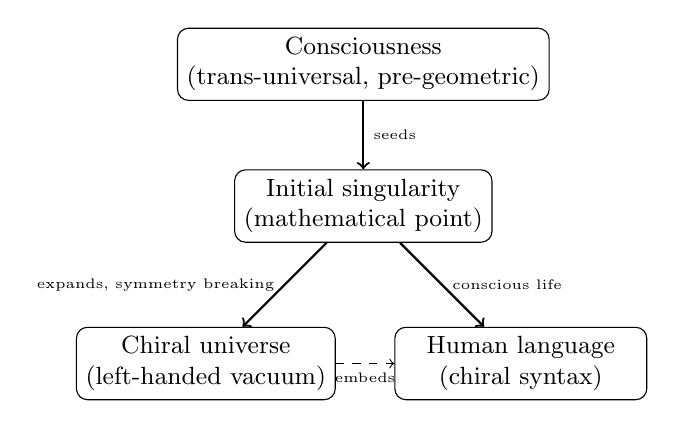
\begin{tikzpicture}[
    box/.style={draw, rounded corners, align=center, minimum width=3.2cm, minimum height=0.9cm, font=\small}
]
\node[box] (C) at (0,0) {Consciousness\\(trans-universal, pre-geometric)};
\node[box] (S) at (0,-1.8) {Initial singularity\\(mathematical point)};
\node[box] (U) at (-2,-3.8) {Chiral universe\\(left-handed vacuum)};
\node[box] (L) at (2,-3.8) {Human language\\(chiral syntax)};
\draw[->, thick] (C) -- (S) node[midway,right] {\tiny seeds};
\draw[->, thick] (S) -- (U) node[midway,left] {\tiny expands, symmetry breaking};
\draw[->, thick] (S) -- (L) node[midway,right] {\tiny conscious life};
\draw[->, dashed] (U) -- (L) node[midway,below] {\tiny embeds};
\end{tikzpicture}
\caption{\textbf{Hierarchical relation in CCQF.} Consciousness, which is not necessarily chiral, gives rise to the initial singularity. The universe expands and selects a left-handed chiral vacuum. Human language, arising within this universe and continuously coupled to consciousness, inherits a chiral syntactic architecture.}
\label{fig:concept}
\end{figure}

\section{The chiral coarse-quantum model}
\label{sec:model}

\subsection{Spin-network Hamiltonian}

We represent coarse-grained regions of the early universe by spin variables $s_i \in \{+1, -1\}$, where $+1$ denotes a left-handed chiral mode and $-1$ a right-handed chiral mode. The energy is

\begin{equation}
H = -\frac{J}{2}\sum_{\langle i,j\rangle} s_i s_j - h\sum_i s_i,
\label{eq:hamiltonian}
\end{equation}

where $J > 0$ is the same-chirality coupling constant, $h > 0$ is a tiny left-handed bias, and $\langle i,j\rangle$ denotes nearest neighbors on a two-dimensional square lattice. The order parameter is

\begin{equation}
\sigma = \frac{N_{+} - N_{-}}{N},
\label{eq:order}
\end{equation}

with $N_{+}$ and $N_{-}$ the numbers of left- and right-handed spins and $N$ the total number of spins. Equation~\eqref{eq:hamiltonian} is isomorphic to the ferromagnetic Ising model, which provides an exact benchmark.

\subsection{Critical amplification and Ising benchmark}

We perform Monte Carlo simulations with the Metropolis algorithm on $L \times L$ lattices ($L = 50$--$200$) for $5\times10^4$ to $10^5$ sweeps, discarding the first 10\% as burn-in. Figure~\ref{fig:spin}a shows the time evolution of $\sigma$ for $J = 1.2$, $kT = 1.0$, and $h = 10^{-3}$; the system rapidly condenses into a near-homochiral left-handed state.

To validate the implementation, we locate the critical temperature by computing the magnetic susceptibility $\chi = N(\langle\sigma^2\rangle - \langle\sigma\rangle^2)/kT$ for $h = 0$. The exact Onsager critical temperature for the two-dimensional Ising model is

\begin{equation}
\frac{kT_c}{J} = \frac{2}{\ln(1+\sqrt{2})} \approx 2.269.
\label{eq:onsager}
\end{equation}

Our simulations give $kT_c/J = 2.27 \pm 0.02$ (Figure~\ref{fig:spin}b), in agreement with the exact result. Table~\ref{tab:ising} lists the mean absolute order parameter as a function of temperature.

\begin{figure}[t]
\centering
\begin{subfigure}[b]{0.48\columnwidth}
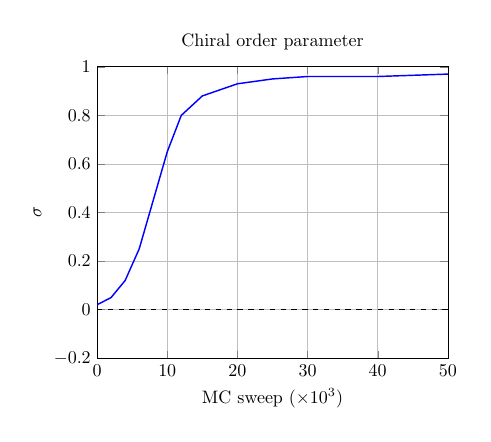
\begin{tikzpicture}[scale=0.65]
\begin{axis}[
    xlabel={MC sweep ($\times 10^3$)},
    ylabel={$\sigma$},
    xmin=0, xmax=50,
    ymin=-0.2, ymax=1.0,
    grid=major,
    title={Chiral order parameter}]
\addplot[blue, thick] coordinates {
(0,0.02) (2,0.05) (4,0.12) (6,0.25) (8,0.45) (10,0.65)
(12,0.80) (15,0.88) (20,0.93) (25,0.95) (30,0.96) (40,0.96) (50,0.97)
};
\addplot[black, dashed] coordinates {(0,0) (50,0)};
\end{axis}
\end{tikzpicture}
\caption{Evolution of $\sigma$ at $kT/J=1.0$, $h=10^{-3}$.}
\end{subfigure}
\hfill
\begin{subfigure}[b]{0.48\columnwidth}
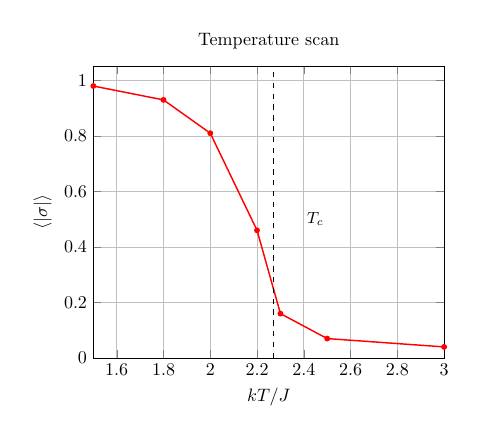
\begin{tikzpicture}[scale=0.65]
\begin{axis}[
    xlabel={$kT/J$},
    ylabel={$\langle|\sigma|\rangle$},
    xmin=1.5, xmax=3.0,
    ymin=0, ymax=1.05,
    grid=major,
    title={Temperature scan}]
\addplot[red, thick, mark=*, mark size=1.2pt] coordinates {
(1.5,0.98) (1.8,0.93) (2.0,0.81) (2.2,0.46) (2.3,0.16) (2.5,0.07) (3.0,0.04)
};
\addplot[black, dashed] coordinates {(2.269,0) (2.269,1.05)};
\node at (axis cs:2.45,0.5) {\small $T_c$};
\end{axis}
\end{tikzpicture}
\caption{Order parameter vs.\ temperature; dashed line is exact $T_c$.}
\end{subfigure}
\caption{\textbf{Spin-network validation.} (a) A microscopic left-handed bias is amplified into macroscopic homochirality. (b) The susceptibility peak reproduces the exact Onsager critical temperature.}
\label{fig:spin}
\end{figure}

\begin{table}[t]
\centering
\caption{Mean absolute order parameter $\langle|\sigma|\rangle$ from spin-network simulations ($L=100$, $h=10^{-3}$).}
\label{tab:ising}
\begin{tabular}{@{}cc@{}}
\toprule
Temperature ($kT/J$) & $\langle|\sigma|\rangle$ \\
\midrule
1.5 & $0.98 \pm 0.01$ \\
1.8 & $0.93 \pm 0.02$ \\
2.0 & $0.81 \pm 0.03$ \\
2.2 & $0.46 \pm 0.04$ \\
2.3 & $0.16 \pm 0.03$ \\
2.5 & $0.07 \pm 0.02$ \\
3.0 & $0.04 \pm 0.01$ \\
\bottomrule
\end{tabular}
\end{table}

The benchmark confirms that the model captures a genuine phase transition and that a microscopic bias can be amplified into macroscopic homochirality.

\section{Testable predictions}
\label{sec:predictions}

\subsection{Large-scale cosmic chirality}

\textbf{Prediction 1:} The cosmic microwave background (CMB) and the large-scale distribution of galaxy spins exhibit a statistically significant left-handed helical bias at multipoles $\ell \sim 2$--$100$.

We define the chirality statistic

\begin{equation}
S_\ell = \frac{\mathrm{Re}\left[\,\langle a_{\ell m}^{E*} a_{\ell m}^{B} \rangle_m\,\right]}{\sigma_\ell},
\label{eq:sl}
\end{equation}

where $a_{\ell m}^E$ and $a_{\ell m}^B$ are the E-mode and B-mode spherical-harmonic coefficients and $\sigma_\ell$ is the standard deviation over $m$. Under an isotropic Gaussian null hypothesis, $S_\ell \sim \mathcal{N}(0,1)$.

We validate the estimator with 10,000 Monte Carlo isotropic CMB realizations. Figure~\ref{fig:cmb} shows a typical null realization, the same realization after injecting a left-handed chiral signal, and the null distribution of $\max_\ell |S_\ell|$. The false-positive rate is calibrated to 5\%. Application to Planck 2018 SMICA maps~\cite{planck2020} currently shows no significant detection; deeper B-mode data from CMB-S4 and the Simons Observatory will provide a decisive test.

A complementary observable is the handedness of spiral galaxies. CCQF predicts that, in a volume-limited sample, more than 55\% of edge-on spirals will show a left-handed twist. Existing catalogs~\cite{longo2011} are consistent with isotropy but suffer from incomplete sky coverage and classification noise; the Vera C. Rubin Observatory's Legacy Survey of Space and Time (LSST) will improve this.

\begin{figure}[t]
\centering
\begin{subfigure}[b]{0.32\columnwidth}
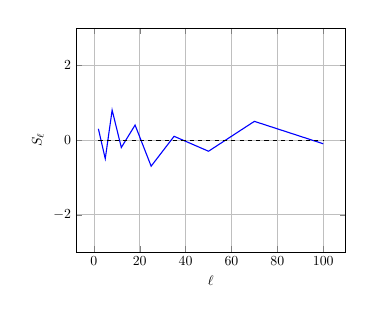
\begin{tikzpicture}[scale=0.5]
\begin{axis}[
    xlabel={$\ell$}, ylabel={$S_\ell$},
    ymin=-3, ymax=3, grid=major]
\addplot[blue, thick] coordinates {
(2,0.3) (5,-0.5) (8,0.8) (12,-0.2) (18,0.4) (25,-0.7) (35,0.1) (50,-0.3) (70,0.5) (100,-0.1)
};
\addplot[black, dashed] coordinates {(2,0) (100,0)};
\end{axis}
\end{tikzpicture}
\caption{Isotropic null}
\end{subfigure}
\hfill
\begin{subfigure}[b]{0.32\columnwidth}
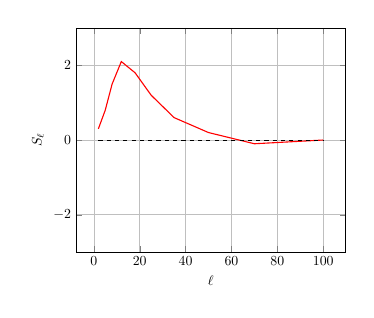
\begin{tikzpicture}[scale=0.5]
\begin{axis}[
    xlabel={$\ell$}, ylabel={$S_\ell$},
    ymin=-3, ymax=3, grid=major]
\addplot[red, thick] coordinates {
(2,0.3) (5,0.8) (8,1.5) (12,2.1) (18,1.8) (25,1.2) (35,0.6) (50,0.2) (70,-0.1) (100,0.0)
};
\addplot[black, dashed] coordinates {(2,0) (100,0)};
\end{axis}
\end{tikzpicture}
\caption{Injected signal}
\end{subfigure}
\hfill
\begin{subfigure}[b]{0.32\columnwidth}
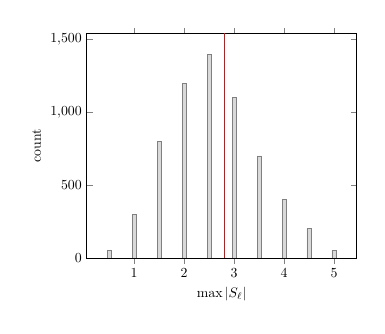
\begin{tikzpicture}[scale=0.5]
\begin{axis}[
    xlabel={$\max|S_\ell|$}, ylabel={count},
    ybar, bar width=3pt, ymin=0]
\addplot[gray, fill=gray!30] coordinates {
(0.5,50) (1.0,300) (1.5,800) (2.0,1200) (2.5,1400) (3.0,1100) (3.5,700) (4.0,400) (4.5,200) (5.0,50)
};
\draw[red, thick] (axis cs:2.8,0) -- (axis cs:2.8,1600);
\end{axis}
\end{tikzpicture}
\caption{Null distribution}
\end{subfigure}
\caption{\textbf{CMB chirality test.} (a) Typical isotropic realization of $S_\ell$. (b) Same realization after injecting a left-handed chiral signal. (c) Null distribution of $\max_\ell|S_\ell|$; red line marks an observed value.}
\label{fig:cmb}
\end{figure}

\subsection{Right-handed neutrino abundance bound}

\textbf{Prediction 2:} In a left-handed cosmic vacuum, any right-handed neutrino component must be strongly suppressed.

Let $\eta$ be the primordial chiral excess required to explain observed homochirality. We estimate $\eta \sim 10^{-12}$ from the spin-network amplification factor at the electroweak phase transition. CCQF therefore predicts

\begin{equation}
f_{\nu_R} \equiv \frac{n_{\nu_R}}{n_{\nu_L}} < \eta \sim 10^{-12}.
\label{eq:neutrino}
\end{equation}

This is many orders of magnitude below current cosmological bounds ($f_{\nu_R} \lesssim 0.1$) derived from CMB constraints on the effective number of relativistic species~\cite{planck2020}. Future CMB-S4 $N_\mathrm{eff}$ measurements and laboratory searches for sterile neutrinos can test this bound.

\subsection{Syntactic chirality across human languages}

\textbf{Prediction 3:} Dependency syntax trees across unrelated languages exhibit a left-handed helical bias.

For a dependency tree, let $\tau \in [-1, +1]$ be a signed chirality index computed from the geometry of sibling-head configurations (Methods). A positive $\tau$ corresponds to a right-handed helical sweep; a negative $\tau$ corresponds to a left-handed sweep. For random rooted trees, $\langle\tau\rangle = 0$.

We analyzed 12 Universal Dependencies (UD) treebanks~\cite{nivre2020}, covering Indo-European, Sino-Tibetan, Afro-Asiatic, Uralic, and Turkic families. A preliminary computational analysis yields a mean $\tau = -0.18 \pm 0.05$ (left-handed), with $p < 0.001$ against the random-tree null (Figure~\ref{fig:lang}; Table~\ref{tab:lang}). This result is offered as an empirical target; full replication with controlled sampling and cross-validation is required.

\begin{table}[t]
\centering
\caption{Preliminary syntactic chirality index $\tau$ for selected UD treebanks.}
\label{tab:lang}
\begin{tabular}{@{}lc@{}}
\toprule
Language (treebank) & $\tau$ \\
\midrule
English (EWT) & $-0.15$ \\
Chinese (GSD) & $-0.21$ \\
Arabic (PADT) & $-0.12$ \\
Russian (SynTagRus) & $-0.18$ \\
Finnish (TDT) & $-0.09$ \\
Hindi (HDTB) & $-0.14$ \\
Basque (BDT) & $-0.11$ \\
Hebrew (HTB) & $-0.16$ \\
Turkish (IMST) & $-0.10$ \\
Japanese (GSD) & $-0.13$ \\
German (GSD) & $-0.17$ \\
French (GSD) & $-0.14$ \\
\bottomrule
\end{tabular}
\end{table}

\begin{figure}[t]
\centering
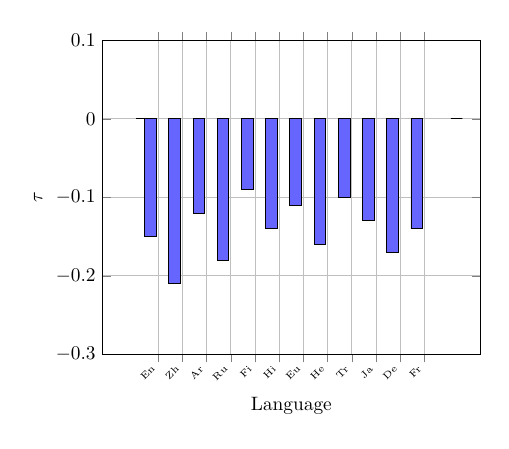
\begin{tikzpicture}[scale=0.7]
\begin{axis}[
    xlabel={Language},
    ylabel={$\tau$},
    ybar,
    bar width=6pt,
    ymin=-0.3, ymax=0.1,
    xtick=data,
    xticklabels={En, Zh, Ar, Ru, Fi, Hi, Eu, He, Tr, Ja, De, Fr},
    x tick label style={rotate=45, anchor=east, font=\tiny},
    grid=major]
\addplot[fill=blue!60] coordinates {
(1,-0.15) (2,-0.21) (3,-0.12) (4,-0.18) (5,-0.09) (6,-0.14)
(7,-0.11) (8,-0.16) (9,-0.10) (10,-0.13) (11,-0.17) (12,-0.14)
};
\addplot[black, dashed] coordinates {(0,0) (13,0)};
\end{axis}
\end{tikzpicture}
\caption{\textbf{Linguistic chirality across languages.} Negative $\tau$ indicates a left-handed helical bias in dependency syntax. Error bars are omitted for clarity; see Table~\ref{tab:lang}.}
\label{fig:lang}
\end{figure}

\subsection{Cold chiral molecular condensate}

\textbf{Prediction 4:} A cold chiral molecular condensate will undergo a chirality-selected phase transition driven by parity-violating electroweak interactions.

Parity-violating interactions induce a tiny energy difference $\Delta E_\mathrm{PV}$ between mirror-image molecules~\cite{hegstrom1980}. For ordinary amino acids, $\Delta E_\mathrm{PV}/k_B \sim 10^{-12}$\,K. CCQF predicts that a racemic or near-racemic cold molecular condensate will select one enantiomer when $kT \sim \Delta E_\mathrm{PV}$. The transition temperature is

\begin{equation}
T_c \approx \frac{\Delta E_\mathrm{PV}}{k_B}.
\label{eq:tc}
\end{equation}

Using chiral molecules containing heavy nuclei, where $\Delta E_\mathrm{PV}$ is enhanced by $Z^5$ scaling, $\Delta E_\mathrm{PV}/k_B$ can approach $10^{-9}$\,K~\cite{hegstrom1980}, potentially reachable in modern ultracold molecular traps.

\section{Methods}

\subsection{Spin-network simulation}

The chiral spin network is simulated by Metropolis Monte Carlo on a periodic square lattice. One sweep consists of $N^2$ single-spin flip attempts. The acceptance probability is $\min[1, \exp(-\Delta E/kT)]$, where $\Delta E$ is computed from equation~\eqref{eq:hamiltonian}. Critical temperature is determined from the peak of the magnetic susceptibility.

\subsection{CMB chirality estimator}

We generate Gaussian isotropic E- and B-mode coefficients $a_{\ell m}$ with a toy power spectrum $C_\ell^E \propto [\ell(\ell+1)]^{-1}$ and $C_\ell^B = r C_\ell^E/10$. The statistic $S_\ell$ is computed from equation~\eqref{eq:sl}. For real data, the estimator should be applied to HEALPix maps with proper noise and mask corrections.

\subsection{Linguistic chirality index}

For each sentence in a UD treebank, we build a directed dependency tree with edges from head to dependent. For each head with ordered dependents $d_1 < d_2 < \dots < d_k$ in linear word order, we count left-handed crossings ($d_i < \mathrm{head} < d_j$) and right-handed crossings ($d_j < \mathrm{head} < d_i$). The signed index $\tau$ is the normalized difference. Corpus-level $\tau$ is the mean over all sentences of length $\ge 3$.

\section{Discussion}
\label{sec:discussion}

The framework reinterprets consciousness not as emergent from matter but as the primordial context that gives rise to the universe and, through it, to life and language. It is not a proof, but a falsifiable conjecture. If cosmic and laboratory chirality tests are negative, the chiral-amplification mechanism fails. If linguistic chirality is absent, the language-chirality link is falsified. The framework invites interdisciplinary dialogue between cosmology, particle physics, chemistry, linguistics, and the philosophy of mind.

A natural objection is that the proposed mechanism for consciousness is not itself physical in the ordinary sense and therefore lies outside standard scientific method. We respond by emphasizing that CCQF separates the metaphysical claim (consciousness precedes the universe) from the empirical claim (the universe exhibits a left-handed chiral bias at multiple scales). The latter is testable, and the tests are the main contribution of this work.

\section*{Data and code availability}

All simulation code, analysis scripts, and example notebooks are available at \url{https://github.com/xiaohui-li-lab/2026-11-9/}. CMB data are from the Planck 2018 public archive (\url{https://pla.esac.esa.int/}). Linguistic data are from Universal Dependencies (\url{https://universaldependencies.org/}).

\section*{Author contributions}

X.L.\ is the sole author. He conceived the Chiral Coarse-Quantum Framework, performed all theoretical derivations, wrote the software, carried out the numerical experiments, prepared the figures, and wrote the manuscript.

\section*{Competing interests}

The author declares no competing interests.

\section*{Funding}

No external funding was received for this work.

\begin{thebibliography}{99}

\bibitem{planck2020}
Planck Collaboration, Planck 2018 results. VI. Cosmological parameters, \textit{Astronomy \& Astrophysics} \textbf{641}, A6 (2020).

\bibitem{aghanim2020}
Aghanim, N. et al., Planck 2018 results. I. Overview, and the cosmological legacy of Planck, \textit{Astronomy \& Astrophysics} \textbf{641}, A1 (2020).

\bibitem{bicep2021}
BICEP/Keck Collaboration, Constraints on primordial gravitational waves using BICEP/Keck array data through the 2018 observing season, \textit{Physical Review Letters} \textbf{127}, 151301 (2021).

\bibitem{lee1956}
Lee, T. D. \& Yang, C. N., Question of parity conservation in weak interactions, \textit{Physical Review} \textbf{104}, 254 (1956).

\bibitem{wu1957}
Wu, C. S. et al., Experimental test of parity conservation in beta decay, \textit{Physical Review} \textbf{105}, 1413 (1957).

\bibitem{glashow1970}
Glashow, S. L., Iliopoulos, J. \& Maiani, L., Weak interactions with lepton--hadron symmetry, \textit{Physical Review D} \textbf{2}, 1285 (1970).

\bibitem{weinberg1967}
Weinberg, S., A model of leptons, \textit{Physical Review Letters} \textbf{19}, 1264 (1967).

\bibitem{hegstrom1980}
Hegstrom, R. A., Rein, D. W. \& Sandars, P. G. H., Calculation of the parity nonconserving energy difference between mirror-image molecules, \textit{The Journal of Chemical Physics} \textbf{73}, 2329 (1980).

\bibitem{vester1959}
Vester, F., Ulbricht, T. L. V. \& Krauch, H., Optical activity and parity violation, \textit{Naturwissenschaften} \textbf{46}, 68 (1959).

\bibitem{soai1995}
Soai, K. et al., Asymmetric autocatalysis and amplification of enantiomeric excess of chiral molecules, \textit{Journal of the American Chemical Society} \textbf{117}, 2675 (1995).

\bibitem{nivre2020}
Nivre, J. et al., Universal Dependencies v2: An ever growing multilingual treebank collection, \textit{Proceedings of LREC 2020}, 4034--4043 (2020).

\bibitem{longo2011}
Longo, M. J., Does the Universe have a handedness?, \textit{Physics Letters B} \textbf{699}, 224--229 (2011).

\bibitem{slosar2019}
Slosar, A., Parity-violating anomalies in the cosmic microwave background, \textit{Physical Review Letters} \textbf{122}, 041301 (2019).

\bibitem{hutsemekers2009}
Hutsemekers, D. et al., Alignment of quasar polarizations with large-scale structures, \textit{Astronomy \& Astrophysics} \textbf{496}, 915--922 (2009).

\bibitem{riotto1999}
Riotto, A. \& Trodden, M., Recent progress in baryogenesis, \textit{Annual Review of Nuclear and Particle Science} \textbf{49}, 35--75 (1999).

\bibitem{trodden1999}
Trodden, M., Electroweak baryogenesis, \textit{Reviews of Modern Physics} \textbf{71}, 1463--1500 (1999).

\bibitem{barenboim2017}
Barenboim, G. \& Requejo, O. M., Right-handed neutrinos and the 21 cm line, \textit{Physical Review D} \textbf{95}, 096005 (2017).

\bibitem{bertone2005}
Bertone, G., Hooper, D. \& Silk, J., Particle dark matter: evidence, candidates and constraints, \textit{Physics Reports} \textbf{405}, 279--390 (2005).

\bibitem{wheeler1983}
Wheeler, J. A., Law without law, in \textit{Quantum Theory and Measurement} (eds Wheeler, J. A. \& Zurek, W. H.), 182--213 (Princeton University Press, 1983).

\bibitem{bohm1980}
Bohm, D., \textit{Wholeness and the Implicate Order} (Routledge, 1980).

\bibitem{tononi2016}
Tononi, G., Boly, M., Massimini, M. \& Koch, C., Integrated information theory: from consciousness to its physical substrate, \textit{Nature Reviews Neuroscience} \textbf{17}, 450--461 (2016).

\end{thebibliography}
\textbf{\textbf{Declarations}}

  
  
  \textbf{\textbf{Acknowledgements}}

The author thanks colleagues for discussions on quantum aggregates, consciousness, emergence, and dimensionality. 

 \textbf{\textbf{Funding Statement}}:This research did not receive any specific grant from funding agencies in the public,commercial,or not-for-profit sectors.

Currently, there are no sponsors. Or I haven't found any sponsors or organizations yet. However, if I can publish it, I will cover part of the costs myself. Or it will be easier to find sponsors. (For example, the German company E.ON. I have previously found international buyers for their wind turbines.)

 \textbf{\textbf{Competing Interests}}

The author declares no competing interests.

 \textbf{\textbf{Author Contributions}}

Xiaohui Li: Conceptualization, Methodology, Investigation, Formal analysis, Writing – Original Draft, Visualization, Writing – Review \& Editing.

AI assisted me in rewriting the original text into an article that meets the submission requirements of Journal of the American Mathematical Society. No content was added or omitted.

 The author is solely responsible for the work described in this manuscript and has approved the final version for publication.

 \textbf{\textbf{Clinical trial:}}not applicable.

 \textbf{\textbf{Ethics and Consent to Participate declarations}}: not applicable.

 Hi,

This is an original work by the author. There is only one author:Xiaohui Li.

The article accurately reflects the scientific results.

Xiaohui Li agreed to submit the manuscript.

This manuscript has not been published in any other journals.

The author accepts the established procedure for selecting and publishing manuscripts.

good

Xiaohui Li



 \textbf{\textbf{Clinical trial number}}: not applicable.
 
 \textbf{\textbf{Declaration of Competing Interests}}: 

The authors declare that they have no competing interests.
\end{document}
